
\newrefsection

%\textbf{B1.a. Extended Synopsis of the scientific proposal}

\chapter{B1.a. Extended Synopsis of the scientific proposal}\label{part1}

\eu{(max 5 pages)}

\eu{The Extended Synopsis should give a concise presentation of the scientific
proposal, with particular attention to the ground-breaking nature of the
research project and the feasibility of the outlined scientific approach.
Describe the proposed work in the context of the state of the art of the field.
References to literature should also be included. References do not count
towards the page limits. It is important that this extended synopsis contains
all essential information including the feasibility of the scientific proposal
since the panel will only evaluate Part B1 at step 1.}

%\section{Long-term vision and ground-breaking nature of the project}

\subsection{Project overview and beyond-state-of-art objectives}

The \project project aims at shedding a new light onto this seemingly simple
question: \emph{How can an artificial agent represents its social environment?
How can it represent the rich, dynamic, (often messy) social situations it
experiences, so as to compare them, reason about them, interpret them, make
decision about them?}

Social situations -- i.e. \emph{temporally and spatially bounded series of
events abstracted by the observer from the on-going flow of social life}, as put
by Garbett in~\cite{garbett1970analysis} -- are a fundamental building block in
social psychology~\cite{argyle1981social}. When specifically looking at
artificial agents like social robots, making sense of these situations is critical:
their level of social cognition depends on their ability to identify, interpret
and interact with the world surrounding
them~\cite{szczepanowski2017computational}, and in particular, correctly
interpret transactions of social signals -- specific events in which an agent
performs a social action aimed at another agent~\cite{pantic2011social}. This
process is known as \textit{situational awareness}, of which
Endsley~\cite{endsley1995theory} defines three levels:\emph{perception},
\emph{interpretation}, and \emph{evaluation}.

While the \emph{perception} of social signals in digital social sciences or by
physical AI systems has been studied in depth (see for instance Pantic et
al.~\cite{pantic2011social}), the \emph{interpretation} and the
\emph{evaluation} of social situations are difficult problems.  Interpretation,
in particular, requires to build and maintain a task-appropriate model of the
situation, and represent it in such a way that a machine can reason about it.
\textbf{\project aims at achieving a breakthrough in this regard,
by introducing the idea of \emph{social embeddings} as a novel and generic mathematical
representation of social environments}. 

Social embeddings represent a paradigm shift for the domain: they open the way
to task-agnostic representation and quantitative measurement of a social
mechanism that was until now mostly relying on qualitative methodologies or
specialized, task-specific models. As such, the results of \project will
\textbf{significantly accelerate the development of generic artifical agents
that are socially-aware}, also \textbf{creating an interdiscplinary bridge}
between the current trends in Machine Learning, and the broad range of
disciplines using data-driven approaches for the study of our social world.


\subsection{Core concept of \project}

Inspired by how Large Language Models (LLMs) are able to encode complex social
semantics, \project is about leveraging these models to introduce
\emph{social embeddings}.

In the context of machine learning, we refer to an \emph{embedding} as a
mathematical representation of a typically high dimension input (for instance,
the pixels of an image) into a lower-dimensional space. Critically, embeddings
are trained to encode the relationships and semantic nuances that might exist in
the original input space. For instance, two pictures of the same face
transformed with an embedding tuned for facial recognition would yield two
vectors that are similar to each other (i.e., close to each other for a given
metric like the usual Euclidian distance). As such, the process of embedding not
only condenses high-dimensional information into a more manageable form but also
captures latent associations that might otherwise remain
obscured~\cite{bengio2009learning}.

Work on embeddings has recently yielded spectacular results in language
processing, with the advent of so-called Large Language Models (like Llama or
GPT). These models relies themselves on text-level embeddings, representing
input text as a numerical
vector~\cite{reimers2019sentencebert,muennighoff2022sgpt}. Importantly, the
resulting embeddings have been shown to effectively encode, for instance,
semantic relatedness between texts~\cite{thakur2021beir}.

Combining social situations and text embeddings, \project aims at creating and
characterising \emph{social embeddings}, i.e. a compact, real-valued numerical
representation (a vector) of a social situation, as experienced by an agent
immersed in that social environment. 
%At their basic level, \emph{social
%embeddings} consist in text descriptions of social situations, viewed from the
%agent's perspective, that are then
%projected in the embedding space by a text embedder.
Indeed, the key insight is that of
exploiting the social knowledge already encoded in the latent space of large
language models like Llama2 or GPT-4. I do so by generating a textual
description of the social environment of the agent (using for instance the
existing perception routines of social robots), and by transforming this
description into a text embedding via a large language model.  By doing so, we
effectively construct a \emph{social embedding}, i.e., a projection of the
social space into a machine-friendly numerical space.

It follows from that construction that, similarly to general text embeddings,
social embeddings encode the \emph{semantics} of the social situation currently
experienced by the agent, facilitating the interpretation of the situation. For
instance, comparing two social situation would become as simple as computing a
distance between their respective embedding vectors
(Figure~\ref{fig:social-embeddings}).


\begin{figure}[H]
    \centering
    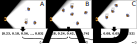
\includegraphics[width=0.9\linewidth]{figs/social-embeddings}
    \caption{General principle of social embeddings~\cite{lemaignan2024social}: arbitrary social situations
    are projected into real-valued vector space, \emph{embedding} their
    semantics. In this example (and assuming the perspective of the yellow
    character), scenes A and B  are more similar to each others (one person
    walking towards the character, with an independent group of people chatting
    in the background), than B and C (in C, the character is already engaged in
    an interaction).  Social embeddings make it possible to e.g. compare such
    social situations using a simple distance between vectors.}

    \label{fig:social-embeddings}
\end{figure}


Formally, if we denote $\mathcal{S}$ the set of social situations, the
\emph{social embedding} process has three steps: (1) a \emph{descriptor
extraction} step $D : \mathcal{S} \to \{\mathcal{D}\}$, with $\mathcal{D}$ the
set of descriptors that can be used to characterise a given social situation
(for instance, relative distances between people, facial expressions, direction
of movement) and its context (e.g. current
location, current task); (2) a \emph{description} step $T: \{\mathcal{D}\}
\to \mathcal{P}$, with $\mathcal{P}$ the set of textual descriptions, that
combines the descriptors into a coherent text-based description of the social
environment; and (3) the embedding process itself $f : \mathcal{P} \to [0;1]^n$,
mapping the textual description to its embedding, i.e. a real-valued vector of
dimension $n$. The text-embedding mapping is a neural network pre-trained on
large datasets of natural language, and optionally fine-tuned to specifically
represent social situations.

The idea of \emph{social embeddings} builds on a proof-of-concept that I already
validated and published~\cite{lemaignan2024social}. \project will take that
early concept, and turn into a mature mathematical tool for social sciences and
artificial social agents. I will fully characterise social embeddings, expand
their scope to complex, real-world social situations, and demonstrate their
transformative potential through deployment of socially intelligent robots in
multiple experimental settings.

%
%The basic idea of \emph{social robots} refers to robots that are situated in a
%human social environment. In this context, we expect social robots to exhibit
%\emph{social awareness}, i.e. to appraise and maintain a model of the social
%situation in which they are embedded. Depending on the role of the robot, this
%might include understanding who is present, who is interacting with whom, which
%are the resulting groups,  what are the in-group roles,  etc.
%
%Social awareness, as a socio-cognitive skill, is essential for the robot to e.g.
%act in a context-sensitive manner; reason and apply social norms (for instance,
%do not navigate in the middle of a group, or do not suddenly interrupt a
%conversation); or create proactive social agents (in order to acknowledge and
%respond to a human who would like to engage with the robot, the robot must first
%adequately model and recognise the corresponding social situation).

%This can only be achieved if robots are endowed with the ability to represent
%not only their physical environment, but also their social environment and
%context. The \project project aims at designing, implementing and characterising
%a radically novel method to achieve this goal, based on the concept of
%\emph{embedding}: a low-dimensional, semantics-preserving, mathematical
%representation of a high-dimensional input (Figure~\ref{fig:social-embeddings}).
%Starting from a proof-of-concept of \emph{social embeddings} that I recently
%published~\cite{lemaignan2024social}, \project develops and fully characterise
%the concept of \emph{social embeddings}, that applies, for the first time, the
%idea of building a compact numerical representation to the complexity of social
%interactions and social dynamics.


%
%At a scientific level, 
%\TODO{articulate scientific impact}
%
%Finally, \project is also about asserting and reinforcing the European
%leadership in AI and intelligent robotics, in line with EU strong societal
%values: a physical AI system able to represent and reason about its social
%environment is also a system that can be designed to have an acceptable and
%positive social impact, in line with the European objectives for socially
%responsible AI. \project can directly contribute to these goals: the science and
%technology that underpins the project \textbf{provide an important contribution
%in securing a safe and responsible digital future in Europe}, as well as
%\textbf{\project building the capacity in Europe to develop socially intelligent
%embodied AI systems}. 

\subsection{Application to Social Robotics}

As a \emph{methodology} to represent and reason about social situations, social
embeddings are fundamentally agnostic from their final domain of application.
However, the practical study and validation of social embeddings does require
experimental grounding, i.e. an artificial social agent embedded into
complex-enough social situations. In \project, I choose to exploit social robots
as an experimental framework.  Beyond my extensive experience and know-how in
social robotics, both at the basic level and at the experimental level, several
scientific and practical reasons drive this choice.

First, compared to many other AI systems (e.g. virtual avatars), robots
are physically situated.  They can partake to a broad range of naturalistic
social situations and social interactions, providing means to acquire,
fine-tune, and validate social embeddings in a variety of real-world scenarios.

Second, not only robots are physically situated, but they also have access to a rich
range of sensing modalities for social perception (including vision, audition).
Combined with robots' proprioception and localisation capabilities, these
percepts can be fully spatially-grounded. This let us compute a rich set of
social constructs (for instance, mutual gaze or joint attention), that feed
directly into the available social descriptors required for social embeddings.

Next, social robots are \emph{active} social agents. From an experimental point
of view, robots' behaviours can be
designed to induce and influence specific social situations, providing us with a
invaluable tool to study social situations and related sociodynamics (see
Objective~\ref{T2}, hereafter).

Finally, beyond the pertinence of social robotics as an \emph{experimental
methodology} for the \project project, the field of social robotics in itself is
``hitting a wall'' \TODO{citation?} to build appropriate tools to represent and
reason about the social environment of robots. By specifically applying social
embeddings to social robotics, I also aim to provide new, groundbreaking
tools to the robotic community to build more intelligent social robots.

\subsection{Objectives beyond state-of-art}

\project is built around three axes: a basic research programme; an experimental
programme that looks specifically at the application of social embeddings to
social robotics; and, running in parallel to those first two axes, a scientific
investigation of the ethical dimension of social embeddings.

At the basic research level, \project targets two overarching research goals:
(1) how to build compact, yet semantics-preserving, embeddings to represent
arbitrary social environments; how to fully characterize these embeddings,
including their latent semantics. I translate this first goal into objective
{\bf O1}:

\begin{enumerate}[label=\textbf{O\arabic*}]
    \item \label{T1} To \textbf{construct and characterize the fundamental
        properties of social embeddings}. This includes researching the three
        steps of embedding generations, including e.g. embedding fine-tuning,
        and the analyse the topology and latent semantics of the social
        embedding space;
\end{enumerate}

\vspace{1em}
\noindent(2) precisely \textbf{frame the socio-cognitive skill of \emph{social awareness} enabled
by social embeddings}, and demonstrate it on social robots. I split this second
goal into three specific objectives:

% 3 objectives:
%- appraise social situations, also taking into account the social context
%- learn socially-appropriate behaviours
%- anticipate future social states


\begin{enumerate}[label=\textbf{O\arabic*}]
    \setcounter{enumi}{1}
    \item \label{T5} To use social embeddings to \textbf{automatically appraise
        social situations}, taking into account their \textbf{context}. Using
        the set of prototypical situations from \ref{T1}, a social embeddings
        can be used to relate the current social situation to known ones.
        Besides, because social embeddings lend themselves to encoding task and
        social context by simply attaching textual descriptions of the context,
        the appraisal of the social situation can be \emph{context-aware};


    \item \label{T4} To \textbf{learn socially-appropriate behaviours} by using
        social embeddings as an additional input feature to existing behaviour
        generation algorithms like Generative Adversarial
        Networks\TODO{citation}; and by augmenting existing interactive machine
        learning techniques (`user in-the-loop' social learning, that I
        pioneered in social robotics~\cite{senft2017supervised,
        winkle2020couch,winkle2021leador}) with representations of the social
        environment;

    \item \label{T2} To use social embeddings to model \textbf{social dynamics}
        by characterizing the trajectories of on-going social situations in the
        embedding space. I will look in particular into trajectories'
        \emph{discontinuties}, that might represent unexpected changes of social
        dynamics, and \textbf{social situation \emph{anticipation}}, by
        extrapolating trajectories in the embedding space;

\end{enumerate}

Once completed, these four objectives will provide solid theoretical and
empirical foundations to social embeddings.

Each of these four objectives involve both basic and experimental research,
presented in the next section.


%%%%%%%%%%%%%%%%%%%%%%%%%%%%%%%%%%%%%%%%%%%%%%%%%%%%%%%%%%%%%%%%%%%%%%%%%%%%%%%

\section{Methodology}
%\section{Feasibility of the project}


The \project project work programme is organised in three main work packages,
that follow each other: the first one, \emph{\wpOne}, focuses on basic research;
the second one, \emph{\wpTwo}, focuses on the artificial socio-cognitive skills
enabled by social embeddings; and the third one, \emph{\wpThree}, specifically
look at the application and impact on social robots.
I briefly describe each of them hereafter, with the key research methods that I
will rely on.

\subsection{WP1: \textbf{\wpOne}}

WP1 addresses Objective \ref{T1}. I will first systematically investigate the
three steps of social embeddings construction, and then characterize the
resulting embeddings.

Social embeddings construction requires first to extract descriptors, then to
build complete textual descriptions, and finally to embed these descriptions.  I
will extract basic social descriptors using the ROS4HRI social perception
approach, as it formalize a multi-modal model of humans~\cite{lemaignan2022ros},
and run in real-time on current robots. I will augment these basic descriptors
with (1) descriptors of human-objects interactions
(HOI), using transformer-based techniques like~\cite{iftekhar2022what}
%, combined with a semantic model of the
%environment, based on~\cite{lemaignan2018underworlds}
; (2) descriptions of the facial expressions based on facial action units
classification~\cite{martinez2019automatic}; (3) group-level
interactions, including $f$-formations, using for instance Hough
voting~\cite{setti2015fformation}, and group activity recognition, using deep
convolutional graph techniques like ARG~\cite{wu2019learning}.

%(3) a novel contextual model of
%attention~\cite{ferrini2024percepts} that allows fine-grained assessment of what
%the person around the robot are focusing on.

The generation of textual descriptions includes both the combination of
descriptors into complete social \emph{snapshots}, and the combination over time
of such snapshots to describe a complete situation. I will initially build
snapshots using text templates, and then extend them using recent techniques
based on social knowledge graphs~\cite{sap2019atomic} and propositional
logic~\cite{tsoi2022sean}. The combination of snapshots into social situations
will be developed with the help of the PHASE simulator and
dataset~\cite{netanyahu2021phase}, that includes a large number of annotated and
longer-horizon social interactions.

Last, the text embedding process itself. Due to the fast pace of progress in the
LLMs landscape, it is likely that current
methods~\cite{reimers2019sentencebert,muennighoff2022sgpt} at time of writing
this proposal will have been replaced by new methods. I will closely monitor
advances in the domain, especially on the question of semantic
relatedness~\cite{thakur2021beir}, as this is critical for social
embeddings. I plan to also perform fine-tuning~\cite{hadsell2006dimensionality}
of the best text embedders to specialize them for social situation
representation. I will do so by leveraging existing open annotated datasets of
social interaction like AMI~\cite{carletta2007ami}, D64~\cite{oertel2013d64},
SALSA~\cite{alameda2015salsa}, or my own SoGrIn dataset~\cite{webb2023sogrin},
and datasets of social questions-answers like SocialIQa~\cite{sap2019social}.

I will then characterise social embeddings, starting with the fundamental
properties that I identified in~\cite{lemaignan2024social}: invariance to
syntax, social similarity and continuity. Next, and of particular interest, is
the question of the embeddings' latent semantics. For instance, we can expect
that social situations like `two persons chatting and laughing together'; or `a
group of three people walking together'; or `one single person walking towards
the robot, looking agitated'; etc.  are all semantically distinct, and,
consequently, would belong to distinct regions in the embedding space.

Identifying such clusters to characterize the semantic topology of the embedding
space~\cite{sun2023topological} will be achieved by exploiting existing datasets
of social interactions (like AMI~\cite{carletta2007ami},
D64~\cite{oertel2013d64}, SALSA~\cite{alameda2015salsa}, or my own SoGrIn
dataset~\cite{webb2023sogrin}), to build and annotate a typology of prototypical
social situations.

\vspace{1em}
\noindent\emph{ Timeframe: Y1-Y3; one post-doc (PD1) with expertise in
    deep learning/text embedding; one post-doc (PD2) in data-driven sociology
signal processing/machine learning/cognitive modelling.}


\subsection{WP2: \textbf{\wpTwo}} 

Work package WP2 focuses on research objectives \ref{T5}, \ref{T4} and \ref{T2}: expanding
social embeddings beyond their fundamental properties, to build a `social
awareness' cognitive skill for social robots.

%\emph{Social awareness} is a socio-cognitive skill that is essential for
%artificial social system, like social robots, to e.g.  act in a
%context-sensitive manner, reason and apply social norms,
%or create proactive social agents (in order to acknowledge and respond to a
%human who would like to engage with the robot, the robot must first adequately
%model and recognise the corresponding social situation).


% METHODS for the 3 objectives?
%- appraise social situations, also taking into account the social context
%- learn socially-appropriate behaviours
%- anticipate future social states


For Objective~\ref{T5}...

Context-awareness is another critical aspect of social situation appraisal.
\emph{Context} has been defined in various way, including as \emph{who},
\emph{what}, \emph{when}, \emph{where}, and \emph{why} of
interactions~\cite{vinciarelli2009social}; as high-level task/environment
characteristics, such as `studying' or `dining'~\cite{nigam2015social}; as
relationships between agents in the scene, such as `interacting in a group',
`standing in a line'~\cite{althaus2004navigation}; or as
task-based~\cite{castellano2012detecting}.

Conceptually, social embeddings lend themselves well to context encoding, as it
simply requires to generate a text description of the situation context (e.g.
location, robot's role, on-going task, etc.), and to insert it into the
social situation description, before performing the text embedding itself.

Using current scene understanding techniques\TODO{cite -> CVUT?} \emph{characterizing} how context impacts the result social embeddings
requires extensive research, from defining and specifying a taxonomy of
contexts, to characterizing their impact on the social embedding space.

\TODO{need to be SMART: reference specific techniques + metrics}


Objective~\ref{T4} and the learning of socially-appropriate behaviour
generation, \project aims at significantly advancing the state of the art in
this regard, by combining two techniques: (1) generative neural networks
for affective robot motion
generation~\cite{marmpena2019generating,suguitan2020moveae}; (2) interactive
machine learning in high-dimensional input/output spaces, where I have shown
with my students promising results for generating complex social
behaviours~\cite{senft2019teaching, winkle2020couch} that fully involve the
end-users~\cite{winkle2018social}. Modulating (1) with the learnt features of
(2), I target a breakthrough in robots' social behaviours generation: the
generation of non-repetitive, socially congruent and transparent social
behaviours (including gestures but also gazing behaviours and facial
expressions).

REgarding interactive machine learning, and building on my previous research on human-in-the-loop social
learning~\cite{senft2017supervised, senft2019teaching,
winkle2020couch,winkle2021leador}, this work package looks into the mechanics to
allow human end-users to progressively teach the robot a domain-specific social
policy, using social embeddings as a key part of the input state of the
Interactive Machine Learning algorithm.

This task also qualitatively researches how human-in-the-loop machine
learning enables a more trustworthy AI system, by involving the end-users in the
creation of the robot behaviours, resulting in explainable behaviours for the
end-users.

\TODO{rephrase}
\TODO{need to be SMART: reference specific techniques + metrics}


Objective~\ref{T2}, finally, is about analysing \emph{social dynamics} by
studying the \emph{trajectories} of social situations in the embedding space.
For instance, the velocity in the embedding space should reflect the rate of
change of a social situation in the physical space; trajectory extrapolation
could be employed by robots to anticipate upcoming social situations;
discontinuities in the embedding space would reflect brutal social changes that
could trigger specific robot behaviours (for instance to acknowledge or attempt
to repair social situations).
\TODO{need to be SMART: reference specific techniques + metrics}


WP2 also include a specific experimental program that aims at setting a new
benchmark for social awareness in social robots. I will adapt to social
robotics~\cite{lemaignan2015mutual} experimental protocols originally designed
by Frith and Happé~\cite{frith1994autism} to investigate social representation
and mental modelling in autistic children.  This protocol include tasks like
distinguishing \emph{happiness} or \emph{sadness} from \emph{surprise}, or
distinguishing \emph{sabotage} from \emph{deception}: these nuances, quite
self-explanatory to experienced social agents, require subtle modelling of the
context and mental state of agents, and, until now, have not been successfully
reproduced on robots. I aim to show that social embeddings offer a generic
methodology to implement this kind of advanced social awareness.


\vspace{1em}
\noindent\emph{Timeframe: Y2-Y4; one PhD student in data-driven sociology
    (PHD1); one post-doc (PD2, shared with WP1)}

\subsection{WP3: \textbf{\wpThree}}



%WP3 will look specifically into two open problems in the
%social robotics community: automatic social engagement appraisal, and
%socially-congruent behaviour generation. Social embeddings have the potential of
%enabling breakthrough for both these problems.
%
%Regarding engagement recognition, social embeddings allows to think of
%engagement in terms of converging trajectories in the embedding space: an agent
%about to engage (and conversely, about to disengage) can be seen as moving
%\TODO{finish}
%

WP2 will run during most of the project. This workpackage will focus on the
practical integration of social embeddings in a larger cognitive architecture
for autonomous social robots. It will effectively enable the experimental
program of \project.

Building on my previous work on cognitive and control architectures for social
robots~\cite{lemaignan2017artificial,lemaignan2015pyrobots,baxter2016cognitive,lemaignan2014challenges,lemaignan2011what},
this task brings together, in a principled manner, the key perceptual (based on
the ROS4HRI framework, available on the TiagoPro robot~\cite{ros2023ros4hri})
and behavioural capabilities of the robot, and will exploit the social
representations generated in WP1 to design a socially-aware behaviour manager.

\TODO{need to be SMART: reference specific techniques + metrics}

\vspace{1em}
\noindent\emph{Timeframe: Y1-Y4; one PhD student (PHD3) in cognitive
    robotics.}


\subsection{WP6: \textbf{\wpSix}}

Finally, and because the development of socially-intelligent robots has
\textbf{complex ethical ramifications} -- including the potential of alienating
human users, \project also includes a strong research component on Responsible
Robotics. In particular, the project will aim to contribute directly to the
roadmaps for Responsible AI and Responsible Robotics, specifically investigating
the interplay between social embeddings, transparency and human agency.


Social embeddings, by enabling artificial systems to model and reason on their
social environment, have the potential of significantly increase the social
competencies of e.g. robots, also raising ethical questions.

I am part of an international working group on Responsible Robotics~\TODO{cite
Dagsthul roadmap arxiv}...

WP6 aims at establishing the conceptual and ethical framework around the idea of
\emph{robot-supported human-human interactions}. It does so by co-creating
patterns of interaction and norms with the general public, using a unique
combination of ethnographic observations and `crowd-sourced' interaction
patterns.

\vspace{1em}
\noindent\emph{Timeframe: Y3-Y5; one senior post-doc (PD3)
with background in ethics of technology and responsible innovation.}


\subsection{WP7: \textbf{\wpSeven}}

The last workpackage groups all the task related to the grant management, as
well as the dissemination and exploitation tasks. Details of the dissemination
and exploitation activities are provided in Part B2 of the proposal.


\subsection{Expertise and Research team}
\label{research-team}

My expertise is primarily centered on cognitive robotics and human-robot social
interaction. My expertise in this field covers a broad spectrum, from basic
research in robotics (for
instance~\cite{lemaignan2014dynamics,lemaignan2015mutual}) and data-driven
socio-psychology
(including~\cite{lemaignan2014cognitive,irfan2018social,winkle2019effective,bartlett2019what}),
to technical contributions (for instance~\cite{lemaignan2010oro,
lemaignan2017artificial, lemaignan2018underworlds}), to extensive experimental
work (see below; for instance~\cite{hood2015cowriter,winkle2020couch,
lemaignan2022social}).

Over the last 4 years, I have re-focalised my work on \emph{data-driven HRI},
contributing several new large datasets of social
interactions~\cite{lemaignan2018pinsoro,sallami2020unexpected,webb2023sogrin},
developing new data analysis
techniques~\cite{bartlett2019what,webb2022measuring}, and demonstrating with my
students new applications of interactive machine learning to social
interactions~\cite{senft2016sparc,winkle2020couch,winkle2021leador}.  In
parallel, I progressively matured the idea of computing compact
\emph{embeddings} of social situations, until I recently published a first
breakthrough in that direction~\cite{lemaignan2024social} (to appear at IEEE/ACM
HRI'24). This ERC project is directly born from this multi-year endeavour
towards data-driven social sciences applied to embodied AI systems, and aims at
significantly accelerate research in this direction.

In particular, \project is the opportunity to gather an interdisciplinary team
of academics that would effectively complement my expertise, and ensure the
feasibility of the project.

Specifically, I intend to recruit:

\begin{itemize}

    \item  two researchers with expertise in data-driven
        socio-psychology (one senior post-doc PD1, one PhD student PHD1); these
        researchers will directly contribute to the human data acquisition,
        the interpretation of social embeddings in term of social situations,
        and the experimental work;

    \item two researchers with expertise in deep machine learning and large
        language models (one senior post-doc PD2, one PhD student PHD2); these
        researchers will contribute to the core implementation of social
        embeddings, including language model fine-tuning, as well as the
        analysis of the embedding space topology;

    \item one research in cognitive robotics (PhD student, PHD3); this
        researcher will focus on the effective integration of social
        embeddings into a larger cognitive architecture for social robots, able
        to autonomously drive interactions;

    \item one researcher in ethics of technology (post-doc
        level PD3); this researcher will lead the work on understanding social
        embeddings in terms of ethical and responsible research.
\end{itemize}

In addition, the host institution (INRIA Grenoble) will provide extensive
additional expertise on machine learning applied to robotics. I will specifically build on
my already established collaboration with Dr. Xavier Almeida-Pineda, head of the
RobotLearn research group. Dr. Almeida-Pineda is the coordinator of the EU H2020
SPRING project on social robotics for geriatric care, on which I collaborated
for the past two years.

Additional expertise, as well as access to one of my main experimental
environment, will be provided through a collaboration with Paris' public
hospitals (APHP) and specifically, with Dr. Maribel Pino, head of research at
Paris' Broca geriatrics hospital (Dr. Pino has extensive experience running
studies with social robots on the hospital' premisses).

%%%%%%%%%%%%%%%%%%%%%%%%%%%%%%%%%%%%%%%%%%%%%%%%%%%%%%%%%%%%%%%%%%%%%%%%%%%%%%%%%%%%
%%%%%%%%%%%%%%%%%%%%%%%%%%%%%%%%%%%%%%%%%%%%%%%%%%%%%%%%%%%%%%%%%%%%%%%%%%%%%%%%%%%%
%%%%%%%%%%%%%%%%%%%%%%%%%%%%%%%%%%%%%%%%%%%%%%%%%%%%%%%%%%%%%%%%%%%%%%%%%%%%%%%%%%%%

\section{Work programme}


\subsection{Ambition of the project}

In addition, social robots are emerging as key enablers to address several
emerging societal challenges, like the ageing society or increasing social
isolation. In this context, not only we lack appropriate tools to model the
social environment of robots, severely limiting their effectiveness, but also
researchers in social robotics have the prime responsibility to ensure that
robots can properly understand and reason about their spatial and social
environment, also ensuring responsible and positive societal impact. As such,
beyond using robots as an experimental methodology, \project also has the
ambition to significantly transform the field of social robotics itself.


\subsubsection{Ambition of the experimental program}

\project experimental program is ambitious. Indeed, each of the project's
research objectives is to be supported experimental work with
a social robot. While some initial studies will be lab-based, most of the later
experimental work will take place in-situ, with real-world users like the
patients of the Broca hospital.

Successful fieldwork with social robots relies on (1) the availability of
the necessary AI algorithm to generate social embeddings and derive robots'
behaviours; (2) the implementation and testing of the software on actual robotic
hardware; (3) the deployment of the robot in real-world public spaces, with the
associated required know-how. Combined with my skills and experience, \project
is designed to effectively and successfully deliver on its experimental program:

Regarding item (1): using publicly available resources, including machine
learning architectures like Transformers, and state-of-art open-source
pre-trained Large Language Models, so-called \emph{foundational models} like
Llama2~\cite{touvron2023llama}, I have shown in~\cite{lemaignan2024social} that
simple social embeddings can indeed already be generated in near-real time on
consumer-grade GPUs. The integration of social embeddings in a larger cognitive
architecture suitable for social robots will require extending existing
robotic architectures, of which I have extensive
experience~\cite{lemaignan2017artificial, lemaignan2015pyrobots,
baxter2016cognitive,lemaignan2014challenges,lemaignan2011what}.

\begin{wrapfigure}[11]{l}{0.15\linewidth}
    \centering
    \vspace{-10pt}
    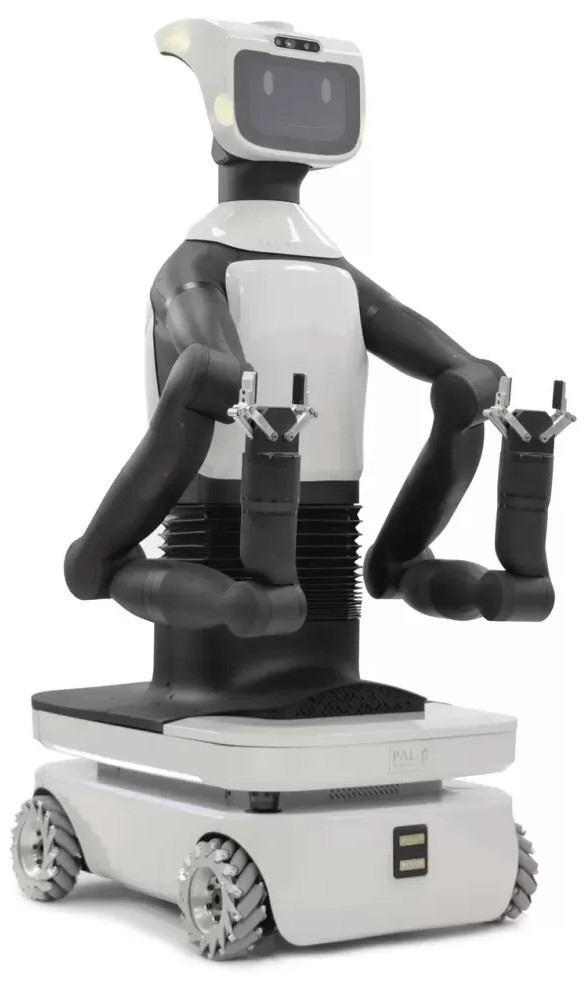
\includegraphics[width=\linewidth]{tiagopro}
    \label{fig|tiagopro}
\end{wrapfigure}

Regarding item (2), the deployment on actual hardware: as \project focuses
specifically on the AI engine of the robot, I will use an existing,
off-the-shelf, social robot (most likely, a PAL Robotics TIAGoPro, pictured on
the left). TIAGoPro offers out-of-the-box advanced human perception based on the
ROS4HRI framework (that I myself originally
designed~\autocite{mohamed2021ros4hri} as an international standard for
Human-Robot Interaction~\autocite{lemaignan2022ros}). It also offers on-board
GPU options that are appropriate to implement a fully AI-based autonomous
system.  I have extensive experience with this platform, having actually
directly taken part to its design and software stack implementation while
employed at PAL Robotics.

Finally, I have an extensive track-record of fieldwork and real-world robot
deployments. From studies in schools~\autocite{hood2015when,
lemaignan2016learning, jacq2016building,
baxter2015wider,kennedy2016cautious,senft2018robots,lemaignan2022social}, at
people's home~\autocite{mondada2015ranger}, in public
spaces~\autocite{alhafnawi2022deliberative}, or in healthcare environments
(including hospitals and care
home)~\autocite{winkle2020couch,cooper2023challenges}, I have led 20+
deployments of social robots in real-world environments, ranging from a few
days, to several weeks~\autocite{jacq2016building,lemaignan2022social} or
months~\autocite{winkle2020couch}.

%The experimental programme of \project includes large data collection. This will
%be facilitated by my collaboration with Paris' APHP, where they already have
%extensive experience in running data collection protocols with robotic
%platforms (involvment in multiple national and European research projects, like
%SPRING, \TODO{complete}).




\newpage

\printbibliography



%\vspace{0.5em}
%\begin{itemize}
%
%    \item What are the conceptual, algorithmic and technical prerequisites to
%        design and implement such an autonomous \& responsible robots? in
%        particular, what social context understanding and (machine) learning
%        architectures are required to \textbf{enable long-term autonomy} and,
%        eventually, \textbf{engagement} between a robot and its end-users?
%
%    \item What are the conditions and methodologies enabling large scale data
%        acquisition of \textbf{real world, user-driven robots behaviours}? How
%        to then train robots to become \textbf{progressively autonomous}?  And
%        ultimately, how to balance \textbf{autonomy} of the robot with the
%        necessary \textbf{behaviour transparency} and \textbf{human oversight}?
%
%    \item What are the public expectations with respect to the role of social
%        robots, and how can we \textbf{collaboratively design}
%        \textbf{autonomous}, yet \textbf{responsible, beneficial, socially
%        acceptable robots}?
%
%\end{itemize}
%
%\vspace{0.5em}
%\noindent From these questions, I derive the following four objectives that are
%the guiding principles of my research program, both in the short term, and at a
%10-15 years horizon:


%\subsection{Work plan outlook}
%
%My research program could begin rapidly, using publicly available resources,
%including machine learning architectures like Transformers, combined with open-source
%pre-trained Large Language Model backbones; and state-of-art HRI tools like
%ROS4HRI~\autocite{mohamed2021ros4hri} to represent in real-time the social
%environment of the robot. While long and complex data collection campaigns would
%have to be organised, and training infrastructure would need to
%be designed, I expect initial results in the first 3 to 5 years.
%
%This is also a long-term vision: on the one hand, the rapid pace of progress
%of technology (novel deep machine learning architectures, novel HRI tools for
%human and scene understanding) continuously opens novel investigation
%venues; one the other hand, the success of my research vision hinges on
%real-world, long-term experimental work: deploying robots in the healthcare
%sector, creating the conditions for adoption by the end-users, running
%long-term deployments with the end-users are long terms aims
%,... these research activities will take
%place over long period of time.

%\subsection{Importance and impact}
%
%My research program has the potential to be groundbreaking: until now,
%autonomous social robots have had little real world success. Experiments and
%deployments have been mostly limited to constrained application domains, where
%rigid action policies (scripts, task planners) could be sufficient. State-of-art
%robots however fail to handle the complexity and unpredictability of real world
%environments (like the ones encountered in the healthcare domain). In addition,
%these systems see poor field adoption due to several factors including
%difficulty of use, wrong expectations, perceived complexity.
%
%This research program is also important: as socially assistive robots quickly
%develop, it is critical to equip ourselves with a deeper understanding and
%intellectual framing of what social robots \emph{could} and \emph{should} be,
%paving the way for their much broader adoption in the coming years: I will
%actively contribute to this aim, by leading the design and implementation of
%socially-intelligent robots that are socially useful, acceptable in the
%long-term, and ethically responsible, but also by furthering my engagement to
%interdisciplinary work, and broad engagement with the society and policy makers.







%%%%%%%%%%%%%%%%%%%%%%%%%%%%%%%%%%%%%%%%%%%%%%%%%%%%%%%%%%%%%%%%%%%%%%%%%




%How this general
%principle translates into specific guidelines and algorithms -- while taking into
%account the principles of a responsible AI -- is the central
%contribution of Work Package 1.

% This socially-driven goal forms what we call a \emph{social
%teleology}. its own goals have this objective can only be achieved if the
%robot is \textbf{socially-driven}: the robot's behaviours must be driven by the
%intention to support positive human-human interactions. 


%I frame these hypotheses with the idea of \textbf{robot-supported human-human
%interactions}, a novel conceptual framework to `think' the future human-robot
%interactions. I will co-construct this framework through large scale public
%engagement: for a whole year, I will deploy the \project robot within the City
%Lab of Bristol's science centre \emph{WeTheCurious}, relinquishing the control
%of the robot to the visitors themselves. Tasked with remotely operating the
%robot to assist fellow visitors, I will accompany them in `inventing by doing' a
%new grammar of social interactions: what does it mean for a robot to help? How
%to do so in the dynamic, messy, environment of a science centre? What are acceptable
%behaviours? Can we see new social norms emerge? At the end of this experiment,
%we expect 1000s of people to have had experienced -- and co-designed -- how
%robots should interact with humans in a positive, helpful way, and each of these
%experiences will contribute to uncovering and designing the basic principles of
%social interaction for robots. This work is the focus of WP1.
%
%While most of the interactions in the science centre will be short-lived, two further
%large scale experiments will take place over the course of the project: a
%one-year experiment in one of Bristol's Special Education Needs (SEN) school,
%helping 250+ children with psycho-social impairments to develop their social
%skills; a second one-year experiment at the Bristol's children hospital, where
%the robot will join one of the wards where 30+ children with long-term conditions
%stay for months, and engage with the children into playful social activities: telling
%stories, triggering group activities with other children, providing additional
%social presence. In both these experiments, the robot behaviours will be
%co-designed with, and learnt from the end-users themselves: nurses, teachers,
%parents, and where possible, the children themselves.
%
%
%\section{Overview of the \project work programme}
%
%Socially intelligent robots require unique, beyond state-of-the-art,
%capabilities to \emph{(1)} understand the social interactions (social
%situation awareness), \emph{(2)} autonomously decide the best course of action for
%short-term and longer-term social influence, and \emph{(3)} perform the
%appropriate social actions and exert said influence in an appropriate,
%responsible manner.
%
%Not only the required technology is itself beyond state-of-the-art (and will be
%researched and integrated in WP2, WP3 and WP4), but the
%interplay between technology, socio-cognitive psychology, privacy and ethics is
%only starting to be researched and understood. \project offers an
%strong vision and an ambitious, evidenced-based, methodology to significantly
%advance our understanding of this multi-faceted problem.
%
%
%\begin{itemize}
%    \item \textbf{O1: conceptual framing} To construct a solid conceptual
%        framing around the multidisciplinary question of responsible human-robot
%        interactions, answering questions like: What should motivate the robot
%        to step in and attempt to help? or: What social norms are applicable to
%        the robot behaviours? Building on the extensive body of work on
%        Responsible AI, I will investigate the basic principles of
%        responsible robot-mediated social interactions, that must form the
%        foundations of a socially useful robot, accepted and used in the long
%        run.  Using user-centred design and participatory design methodologies,
%        I will identify the determinants and parameters of a responsible social
%        intervention, performed by a socially-driven robot, and formalise them
%        in practical principles.
%
%    \item \textbf{O2: physical-social representation and reasoning} To
%        effectively and responsibly interact with its environment, the robot
%        must first build a comprehensive and continuously updated model, from its
%        spatial and physical configuration, to its social dynamics. I will
%        design and develop a novel cognitive capability of artificial
%        \emph{social situation assessment} to enable the robot to represent
%        real-time social dynamics in its environment. I will achieve this
%        breakthrough by combining existing model-based approaches \TODO{refs}
%        (including my recent research on social state modeling \TODO{refs}, with
%        the expressive power of the new \emph{social embeddings} that I have
%        recently introduced.
%
%    \item {\bf O3: goal-driven, responsible decision making} I aim to create
%        robot behaviours that are perceived as purposeful and intentional
%        (long-term goals), while being shaped by a user-created and
%        user-controlled action policy.  I will integrate long-term social goals,
%        arising from the interaction principles of \textbf{O1}, with the social
%        modeling capability of \textbf{O2}, into a principled, goal-driven
%        cognitive architecture, with responsible AI guarantees. The breakthrough
%        will come from combining these long-term social goals with bottom-up
%        action policies, designed and learnt from the end-users using
%        human-in-the-loop attention-based machine learning.
%
%        I want to specifically test the following two hypotheses: first, that
%        long-term social goals, if suitably co-designed with the public and
%        stakeholders and properly integrated into the robot as a \emph{social
%        teleology}, will create the perception that the robot is intentional and
%        purposeful. This will in turn elicit sustained engagement from its human
%        users.
%
%        Second, that human-in-the-loop machine learning can be used to ensure an
%        additional layer of human oversight and a level of behavioural
%        transparency.  Human-in-the-loop reinforcement learning -- as
%        implemented in the SPARC approach that I have developed with my students
%        and already used in complex social
%        environments~\parencite{senft2017supervised,senft2019teaching,winkle2020insitu}
%        -- relies on an end-user `teacher'. This teacher initially fully
%        controls the robot (via teleoperation) while it learns the action
%        policy, and then progressively relinquishes control up to a point where
%        the robot is effectively autonomous. As I previsouly argued
%        in~\textcite{senft2019teaching}, this approach leads to increased
%        control and ownership of the system, and as a result, increased trust
%        from the end-users.
%
%
%    \item{\bf O4: ambitious field research} Finally, the last major objective of
%        my research project is to demonstrate the effectiveness of my approach
%        in complex, real-world conditions. This means deploying the socially
%        interactive robots in existing social \emph{ecosystems} that are
%        sufficiently complex and open to explore novel social interactions. My
%        objective is also to show that this real-world deployment can be
%        successfully driven by the `end-to-end' involvement of all the end-users
%        and stakeholders: from defining the robot's role, from the different
%        perspective of each end-user, to actually designing and `teaching' the
%        robot what to do.
%
%
%\end{itemize}


